\subsection{可分扩张}

设 K 是一个域。由于 K 的任何扩张都是 K-代数，定义1（V，第119页）中引入的可分性概念特别适用于 K 的扩张的情形。由例3（V，第119页），该可分性定义在代数扩张的情形与 § 7（V，第36页，定义1）中的定义一致。

命题6. --- 域 K 的每个纯扩张都是可分的。

这立即由例1（V，第119页）和命题4（V，第120页）得出。

命题7. --- 设 E 是一个域，G 是 E 的一个自同构群，K 是 E 中由 G 的不变元组成的子域。则 E 是 K 的可分扩张。

设 L 是 K 的一个扩张；存在 L 的一个代数闭扩张 \(\Omega\) ，其在 K 上的超越次数至少等于 E 在 K 上的超越次数。由推论1（V，第117页），存在一个 K-同态 \(u\) （从 E 到 \(\Omega\) 的）。我们用 \(v\) 表示 \(\Omega\) -代数同态（从 \(\mathbf{A} = \Omega \otimes_{\mathbf{K}} \mathbf{E}\) 到 \(\Omega\) 的），它把 \(\lambda \otimes x\) 映为 \(\lambda \cdot u(x)\) （对 \(\lambda \in \Omega\) 和 \(x \in \Omega\) ）；我们记 \(\mathfrak{a}\) 为 \(v\) 的核。

对每个 \(s \in G\) ，设 \(h_s\) 是自同构 \(\operatorname{Id}_{\Omega} \otimes s\) （ \(\Omega\) -代数 \(A\) 的）；同态 \(v \circ h_s\) （从 \(A\) 到 \(\Omega\) 的）的核是素理想 \(\mathfrak{a}_s = h_s^{-1}(\mathfrak{a})\) （ \(A\) 的）。显然，理想 \(\mathfrak{b} = \bigcap_{s \in G} \mathfrak{a}_s\) （ \(A\) 的）在自同构

\(h_{s}\) 下稳定。因此（V，第63页，推论）理想 b 具有形式 \(c \otimes_{K} E\) ，其中 c 是 \(\Omega\) 的一个理想。现在 \(b \subset a \neq A\) ，故 \(c \neq \Omega\) ；由于 \(\Omega\) 是一个域，我们有 c = 0，从而 b = 0。

于是 A 的素理想族 \((\mathfrak{a}_{s})_{s\in G}\) 的交为零。由命题2（V，第118页），该环是既约的，从而其子环 \(L\otimes_{K}E\) 更是如此。由于 L 是 K 的任意扩张，这就证明了 E 在 K 上是可分的。

命题8. --- 设 L 是域 K 的一个扩张。若 L 在 K 上可分，则 L 的每个子扩张都在 K 上可分。反之，若 L 的每个有限生成子扩张都在 K 上可分，则 L 在 K 上可分。

这立即由命题3的 a) 和 b)（V，第119页）得出。

因此可分性可以称为一种具有“有限特征”的性质。

命题9. --- 设 L 是域 K 的一个扩张，M 是一个交换 L-代数（例如 L 的一个扩张）。若 M 在 L 上可分且 L 在 K 上可分，则 M 在 K 上可分。

设 \(K'\) 是 K 的一个扩张。由于 L 是 K 的可分扩张，环 \(K' \otimes_K L\) 是既约的；由于 M 是可分 L-代数，命题5（V，第120页）表明环 \((K' \otimes_K L) \otimes_L M\) 是既约的。现在环 \(K' \otimes_K M\) 同构于 \((K' \otimes_K L) \otimes_L M\) （II，第278页，命题2），因此是既约的。这就证明了 M 在 K 上是可分的。

\pandocbounded{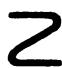
\includegraphics[keepaspectratio]{images/part002_8e27f267.jpg}}

若扩张 M 在 K 上可分，它在 L 上未必可分（但参见 V，第124页，推论3）。例如，若 p 是一个素数，则有理分式域 \(\mathbf{F}_{p}(\mathbf{X})\) （域 \(F_{p}\) 上一个未定元 X 的）在 \(F_{p}\) 上是可分的（V，第121页，命题6），但它是 \(\mathbf{F}_{p}(\mathbf{X}^{p})\) 的一个 p-根式代数扩张；特别地， \(\mathbf{F}_{p}(\mathbf{X})\) 在 \(\mathbf{F}_{p}(\mathbf{X}^{p})\) 上不是可分的。

稍后（V，第137页，命题5）我们将研究复合扩张的可分性。
% semantic-fragments: legacy-input-seam
\relax{}
